\documentclass[12pt]{article}
\usepackage[italian]{babel}
\usepackage{graphicx}
\usepackage[section]{placeins}
\usepackage{amsmath}
\usepackage{enumitem}
\usepackage{subfigure}
\usepackage{listings}
\usepackage{hyperref}
\usepackage{tcolorbox}

\tcbuselibrary{theorems}

\newtcbtheorem[number within = section]{definition}{\emph{Definition }}{colback = gray!10, colframe = gray!50!black, fonttitle = \bfseries}{th}
\newtcbtheorem[]{theorem}{\emph{Theorem }}{colback = gray!10, colframe = gray!50!black, fonttitle = \bfseries}{th}

\title{Geospatial Data Management Project}
\author{
\begin{tabular}[t]{c@{\extracolsep{8em}}c} 
Giuseppe Maurizio Facchi  & Gregorio Ghidoli \\
mat. 989910 & mat.  \\ 
\end{tabular}
}

\date{A.A. 2021-2022}

\begin{document}
\maketitle
\newpage
\tableofcontents
\newpage
\section{Introduzione}
\begin{definition}{Traiettoria}{}
    Una traiettoria è una traccia generata da un oggetto in movimento in spazi geografici, di solito rappresentata da una serie di punti cronologicamente ordinati $$p_1 \rightarrow p_2 \rightarrow \dots \rightarrow p_n$$ dove ogni punto consiste in una coppia di coordinate geografiche associate ad un timestamp $$p=(x,y,t)$$
\end{definition}
Le traiettorie offrono la possibilità di estrarre informazioni da oggetti in movimento, come animali, veicoli o persone.\\
In base alla natura dei dati è possibile classificare le tipologie di dati relative a traiettorie in 4 possibili gruppi (Yu Zheng):
\begin{itemize}
    \item \textbf{Mobilità di persone}
    \item Mobilità di veicoli
    \item Mobilità di animali
    \item Mobilità di fenomeni naturali
\end{itemize}
Il dataset in analisi tratta dati relativi a mobilità di persone, dove 3 visitatori di un museo hanno visto registrare \textbf{attivamente} i loro movimenti per un certo periodo di tempo con un RTLS.
\begin{definition}{RTLS}{}
    Si definisce RTLS qualsiasi sistema (hardware + software) in grado di campionare accuratamente la posizione di un'entità in uno spazio definito ad un'alta frequenza.\\
    RTLS non è uno specifico tipo di sistema, ma più un obiettivo che può essere raggiunto utilizzando vari sistemi (Damiani)
\end{definition}
I real-time location systems utilizzati forniscono la posizione di un tag. In base alle caratteristiche del sistema una posizione può indicare:
\begin{itemize}
    \item \textbf{Presenza} in un'area, espressa simbolicamente
    \item \text{Posizione precisa}, espressa in coordinate
    \item \text{Vicinanza} ad un altro tag, espressa come distanza o simbolicamente
\end{itemize}
Nel caso in analisi la posizione è espressa in coordinate con CRS ESPG 3003.\\[12pt]
Si parla in particolare di registrazione \textbf{attiva} (Yu Zheng) quando l'entità tracciata partecipa direttamente all'attività di tracciamento tramite l'utilizzo di RTLS, come nel caso delle persone in analisi.
\subsection{Paradigma di data mining su traiettorie}
L'operazione relativa all'estrarre informazioni che arricchiscano la conoscenza del dominio di un problema prende il nome di \textit{data mining}. Una possibile organizzazione di tutte le operazioni presenti in letteratura è specificata nella seguente figura, che presenta un paradigma per il \textit{trajectory data mining}.
\begin{figure}[htb!]
    \centering
    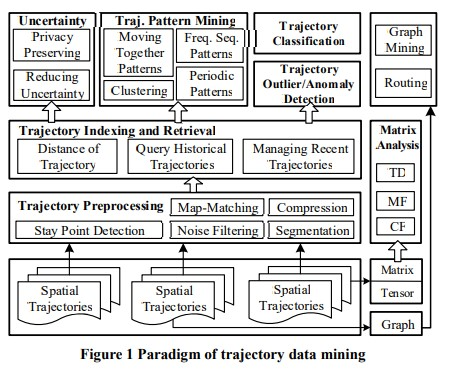
\includegraphics[width=0.8\textwidth]{images/datamining.jpg}
\end{figure}
\FloatBarrier
\subsection{Analisi del dataset}
Il dataset fornito contiene i dati relativi alle esposizioni di un museo (Figura 1) e relativi al tracciamento di 3 persone al suo interno (Figura 2).
\\[12pt](Figura) (caption I dati sono stati forniti come shapefile ESRI e successivamente importati in QGIS, dando il risultato in figura)\\[12pt]
Il tracciamento è stato effettuato per una durata di circa 10 minuti ad una frequenza di campionamento di circa 12 campioni/secondo (1 ogni 0.08 secondi). Una prima analisi è stata effettuata per ricavare le principali statistiche riguardanti le traiettorie di ogni persona, ottenendo i seguenti risultati:
\begin{table}[!ht]
    \centering
    \begin{tabular}{|l|l|l|l|l|}
        \multicolumn{5}{c}{\textbf{\textit{Persona 57}}}                                                                                                                                             \\
        \cline{2-5}
        \multicolumn{1}{l|}{} & \multicolumn{1}{c|}{\textbf{Distanza}} & \multicolumn{1}{c|}{\textbf{Durata}} & \multicolumn{1}{c|}{\textbf{Velocità}} & \multicolumn{1}{c|}{\textbf{Turning Angle}} \\
        \hline
        \textbf{Media}        & 0.040                                  & 0.085                                & 0.485                                  & 185.9                                       \\
        \hline
        \textbf{Mediana}      & 0.030                                  & 0.072                                & 0.374                                  & 182.0                                       \\
        \hline
        \textbf{Minimo}       & 0.000156                               & 0.0709                               & 0.00218                                & 0.01                                        \\
        \hline
        \textbf{Massimo}      & 0.575                                  & 0.179                                & 4.178                                  & 359.9                                       \\
        \hline
        \multicolumn{1}{l}{}  & \multicolumn{1}{l}{}                   & \multicolumn{1}{l}{}                 & \multicolumn{1}{l}{}                   & \multicolumn{1}{l}{}                        \\
        \multicolumn{5}{c}{\textbf{\textit{Persona 67}}}                                                                                                                                             \\
        \hline
        \textbf{Media}        & 0.052                                  & 0.089                                & 0.613                                  & 176.8                                       \\
        \hline
        \textbf{Mediana}      & 0.039                                  & 0.072                                & 0.454                                  & 181.6                                       \\
        \hline
        \textbf{Minimo}       & 0.0006                                 & 0.071                                & 0.003                                  & 0.002                                       \\
        \hline
        \textbf{Massimo}      & 0.493                                  & 0.179                                & 6.226                                  & 359.9                                       \\
        \hline
        \multicolumn{1}{l}{}  & \multicolumn{1}{l}{}                   & \multicolumn{1}{l}{}                 & \multicolumn{1}{l}{}                   & \multicolumn{1}{l}{}                        \\
        \multicolumn{5}{c}{\textbf{\textit{Persona 68}}}                                                                                                                                             \\
        \hline
        \textbf{Media}        & 0.045                                  & 0.087                                & 0.546                                  & 183.3                                       \\
        \hline
        \textbf{Mediana}      & 0.034                                  & 0.072                                & 0.417                                  & 183.2                                       \\
        \hline
        \textbf{Minimo}       & 0.00078                                & 0.071                                & 0.010                                  & 0.006                                       \\
        \hline
        \textbf{Massimo}      & 0.791                                  & 5.356                                & 10.988                                 & 359.9                                       \\
        \hline
    \end{tabular}
    \caption{Dati aggregati relativi alle traiettorie delle persone}
\end{table}
\FloatBarrier
Questi dati verranno utilizzati per inizializzare nel modo migliore gli algoritmi proposti.
\subsection{Obiettivi}
Date le traiettorie, gli obiettivi dell'analisi sono:
\begin{itemize}
    \item Trovare i punti di fermata delle persone (\textbf{stop points})
    \item Data un'esibizione, calcolare il tempo di visita totale nei suoi pressi, considerando solo i punti di fermata
    \item Trovare il numero di persone che in un certo periodo temporale si trovano nei pressi della stessa esibizione
\end{itemize}
\begin{definition}{Punto di Fermata - Stop Point}{}
    Viene generalmente definito "punto di fermata", un punto nel dominio spazio-temporale dove un'entità risulta essere stazionaria. Esistono tipicamente due condizioni di stazionarietà:
    \begin{itemize}
        \item L'entità rimane ferma nello stesso punto per un certo periodo di tempo
        \item Definita un'area, l'entità rimane all'interno di essa per un certo periodo di tempo
    \end{itemize}
\end{definition}
\newpage
\section{Trajectory Preprocessing}
L'operazione di stop point detection e l'operazione di segmentazione della traiettoria fanno parte di quelle operazioni eseguite prima di effettuare ulteriori analisi sul dataset che vengono chiamate di \textit{trajectory preprocessing}:
\begin{figure}[htb!]
    \centering
    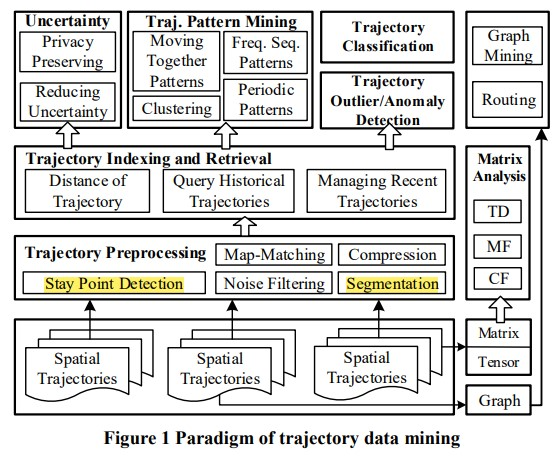
\includegraphics[width=0.8\textwidth]{images/spd.jpg}
\end{figure}
\FloatBarrier
\subsection{Stop points detection}
In letteratura sono presenti diversi algoritmi per l'individuazione dei punti di fermata e conseguentemente per la segmentazione della traiettoria in diversi gruppi di stop. Per questo dataset sono stati presi in considerazione 3 algoritmi che seguono 3 diversi approcci:
\begin{itemize}
    \item Slgoritmo basato su time-space threshold
          %(https://www.researchgate.net/publication/221607181_Project_Lachesis_Parsing_and_Modeling_Location_Histories)
    \item Algoritmo basato su clustering
          %(https://www.mdpi.com/2220-9964/5/3/29)
    \item Algoritmo basato su modelli probabilistici
          %(https://periodicos.ufmg.br/index.php/jidm/article/view/418)
\end{itemize}
\subsubsection{Algoritmo basato su time-space threshold}
\subsubsection{Algoritmo basato su clustering}
\subsubsection{Algoritmo basato su modelli probabilistici}
\subsubsection{Confronto tra gli algoritmi}
\newpage
\section{Trajectory Pattern Mining}
Un importante punto di analisi riguarda il trajectory pattern mining, ovvero l'estrazione di pattern che arricchiscano l'informazione contenuta in una traiettora. Lo scoprire gruppi di persone che si muovono insieme per un certo periodo di tempo ne è un tipico esempio e prende il nome di \textit{moving together pattern}:
\begin{figure}[htb!]
    \centering
    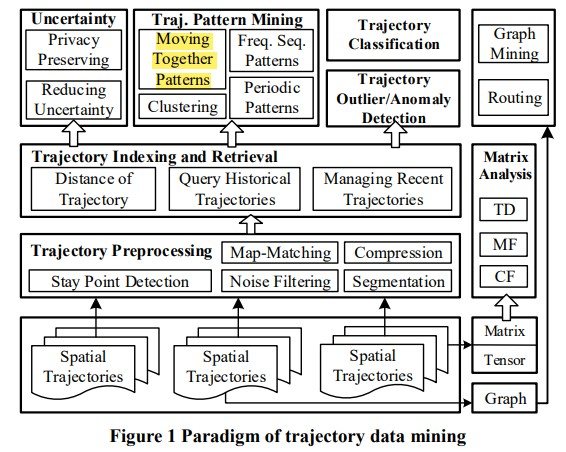
\includegraphics[width=0.8\textwidth]{images/mtp.jpg}
\end{figure}
\FloatBarrier
\subsection{Obiettivo 2}
Partendo dai punti di stop è possibile seguire due differenti approcci per calcolare il tempo totale di visita per ogni esibizione:
\paragraph{Approccio 1} Assegnare ad ogni stop point l'esibizione più vicina considerando il suo centroide, presneta ambiguità per punti tra le intersezioni dei buffer delle exhibit
\begin{enumerate}
    \item Creo buffer delle exhibit e calcolo il centroide
    \item Assegno ogni stop point all'exhibit più vicina in base alla distanza minima tra stop point e centroide di ogni exhibit
    \item Calcolo del visiting time per ogni exhibit
\end{enumerate}
\paragraph{Approccio 2} Assegnare ogni stop point al centroide degli stop points dello stesso segment
\begin{enumerate}
    \item Creo buffer delle exhibit e calcolo il centroide
    \item Calcolo i centroidi del convex hull di ogni segmento di stop points
    \item Considero solo i centroidi che intersecano il buffer delle exhibit e ne calcolo la distanza dal centroide di ogni exhibit
    \item Filtro i risultati ottenuti mantenendo solo le coppie ($C_{sps}$, $C_{exh}$) che presentano la distanza minima
    \item Assegno ad ogni segment l'esibizione più vicina, ottenendo quindi per ogni stop point l'esibizione a cui si riferisce
    \item Calcolo del visiting time per ogni exhibit
\end{enumerate}
\subsection{Obiettivo 3}
Per trovare il numero di persone che in un certo periodo temporale si trovano nei pressi della stessa esibizione è stato utilizzato MobilityDB (ref).\\
In particolare:
\paragraph{Approccio 1}
\begin{enumerate}
    \item Creo buffer delle exhibit e calcolo il centroide
    \item Assegno ogni stop point all'exhibit più vicina in base alla distanza minima tra stop point e centroide di ogni exhibit
    \item Tramite l'utilizzo della funzione $\text{tgeompoint\_seq}$, dai singoli punti sono state create le traiettorie come tipo nativo di MobilityDB
    \item Sono stati raggruppati i risultati per persona ed exhibit contando il numero di persone che in un certo periodo temporale si trovano nei pressi della stessa esibizione
\end{enumerate}
\paragraph{Approccio 2}
\begin{enumerate}
    \item Creo buffer delle exhibit e calcolo il centroide
    \item Calcolo i centroidi del convex hull di ogni segmento di stop points
    \item Considero solo i centroidi che intersecano il buffer delle exhibit e ne calcolo la distanza dal centroide di ogni exhibit
    \item Filtro i risultati ottenuti mantenendo solo le coppie ($C_{sps}$, $C_{exh}$) che presentano la distanza minima
    \item Tramite l'utilizzo della funzione $\text{tgeompoint\_seq}$, dai singoli punti sono state create le traiettorie come tipo nativo di MobilityDB
    \item Sono stati raggruppati i risultati per persona ed exhibit contando il numero di persone che in un certo periodo temporale si trovano nei pressi della stessa esibizione
\end{enumerate}
\end{document}